\documentclass[10pt,compress]{beamer}
\useoutertheme{miniframes}
\usepackage[english]{babel}
%\usepackage[margin=1in]{geometry}

\usepackage{amsmath}
\usepackage{amsfonts} 
\usepackage{amssymb}
\usepackage{amsthm}
\usepackage{mathtools}

\usepackage[utf8]{inputenc}
%\usepackage[exscale, amsfonts, amssymb]{concmath}
%\renewcommand*{\bfseries}{\mdseries}

\usepackage{float}
\usepackage{graphicx}
\usepackage{caption}
\usepackage{subcaption}

\graphicspath{{./src/figures/}}

%\usepackage{fancyhdr} %custom headers and footers layout
\usepackage{lastpage} %package to print the last page
%\pagestyle{fancy} %fancy page style

\usepackage{textcomp} 
\usepackage{multicol} 
\usepackage{multirow}

\usepackage[table]{xcolor}
\usepackage{booktabs}

\usepackage[backend=biber,
bibstyle=ieee, 
citestyle=numeric-comp,
natbib=true,
doi=false, 
url=false,
isbn=false,
mincitenames=1,
maxcitenames=1,
minbibnames=1,
maxbibnames=99,
backref=false,]
{biblatex}
\addbibresource[label=main]{./src/references.bib}

\usepackage{url}
\usepackage{hyperref}

%edit the properties of your PDF documents which will be displayed
\hypersetup{
    bookmarks=true, 		% show bookmarks bar?
    unicode=true,  		% non-Latin characters in Acrobat’s bookmarks
    pdftoolbar=true,        % show Acrobat’s toolbar?
    pdfmenubar=true,        % show Acrobat’s menu?
    pdffitwindow=true,      % page fit to window when opened
    pdftitle={PhotoElectrochemistry --- Theoretical Background},    % title
    pdfauthor={M. Skocic},     % author
    pdfsubject={},   % subject of the document
    pdfnewwindow=true,      % links in new window
    pdfkeywords={}, % list of keywords
    colorlinks=false,       % false: boxed links; true: colored links
    linkcolor=red,          % color of internal links
    citecolor=green,        % color of links to bibliography
    filecolor=magenta,      % color of file links
    urlcolor=cyan           % color of external links
}

\usepackage{tikz}
\usepackage{circuitikz}
\usetikzlibrary{decorations.pathmorphing,arrows,calc}

\title{PhotoElectroChemistry for Corrosion}
\author{M. Skocic, PhD Electrochemistry and Materials}
\date{\vfill 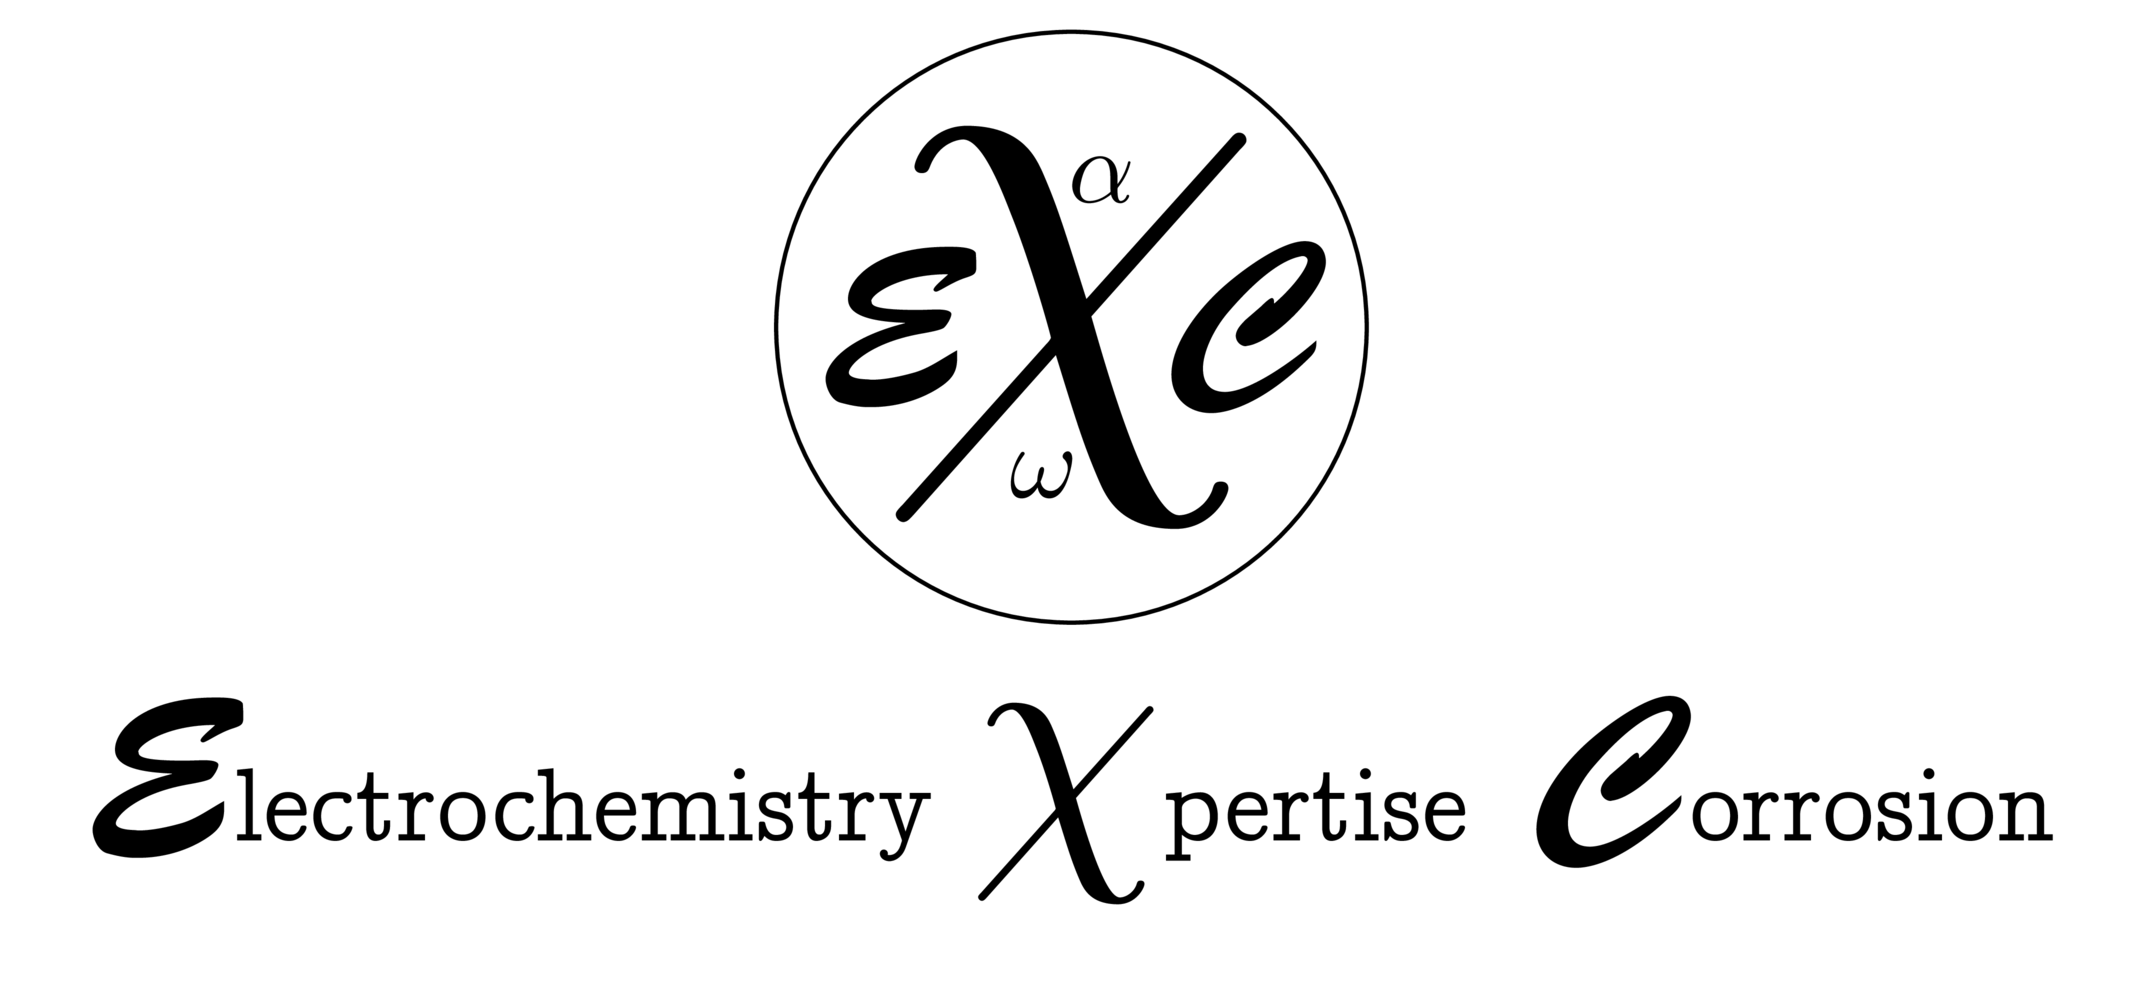
\includegraphics[width=0.70\textwidth]{full_bw.png}}

\begin{document}

\begin{frame}
    \titlepage
\end{frame}

\begin{frame}
    \frametitle{Contents}
    \tableofcontents
\end{frame}



\section{Introduction}
    \begin{frame}{Introduction}
        \begin{itemize}
            \item Photoelectrochemical techniques have been shown to be useful tools for characterizing oxidation layers. 
            \item Interdisciplinary theoretical underpinnings were built \citep{morrison1980, vijh1969, stimming1986, diquarto1997, wouters2007} 
                  such as the Gärtner-Butler model \citep{gartner1959,butler1977}
                  which has been proven to be a simple and robust model for the photocurrent generation. 
            \item Technical progresses were achieved, allowing to study oxide layers at 
                  macroscopic, mesoscopic, and microscopic scales 
                  \citep{benaboud2007, srisrual2011}, or in-situ in high temperature corrosion 
                  conditions \citep{bojinov2002,skocic2016}.
        \end{itemize}
    \end{frame}

    \begin{frame}{Hypotheses}
        Several hypotheses are needed in order to apply the theoretical concepts:  
        \begin{itemize}
            \item semiconductors are considered to be ideal i.e. crystallized and homogeneous  
            \item the dielectric constant of the semiconductor is independent of the light wavelength  
            \item the capacity of the Helmholtz layer is greater than the capacitance of the space charge capacitance  
            \item the potential drop in the Helmholtz layer is independent of the applied potential and is negligible
        \end{itemize}

        \footnotesize
        \begin{alertblock}{Warning}
            The hypotheses are rarely fully respected in the case of oxides or passive 
            films formed on industrial alloys. Nonetheless, the literature shows that the 
            developed models can be applied to non-ideal systems such as oxides 
            and passive films.
        \end{alertblock}
    \end{frame}




\section{basics}
\subsection{Electronic Band Structure}
    \begin{frame}[allowframebreaks=1.0]{Band Model}
        \begin{itemize}
            \item Solids: conductors, semiconductors and insulators. 
            \item Valence and conduction bands correspond to allowed energy states for the electrons. 
            \item $E_c$ is the lowest energy level of the conduction band.
            \item $E_v$ is the highest energy level of the valence band.
            \item $E_g$ is the band gap with no allowed energy states. 
            \item $E_F$ is the Fermi Level which describes the distribution of the electrons among both bands.
        \end{itemize}
        
        \begin{alertblock}{Fermi Level}
            \footnotesize
            The Fermi Level represents the highest energy state that can be occupied level at 0K. 
            It is equivalent to the electrochemical potential in solid phases.
        \end{alertblock}
        
        \framebreak
        \begin{itemize}
            \item The electronic conduction = movement of electrons and/or holes in conduction/valence band.
            \item The conduction depends on the number of available charge carriers
            in the conduction band and in the valence band. 
            \item In conductors: overlap of the conduction and the valence bands occurs. 
            \item In semiconductor and insulator: the conduction depends on the band gap and the energy provided by 
            the environment to the electrons from the valence band in order to jump 
            into the conduction band.
        \end{itemize}

        \begin{circuitikz}[scale=1.0]
\small
\draw[->] (0,-3) -- ++(0,6);
\node[anchor=center, rotate=90] at (-0.25,0) {Electron Energy};

\draw[dashed, thick] (0,0) -- ++(10,0);
\node[draw=none, anchor=south] at (5,0.2) {Fermi Level: $E_F$};

\node[rectangle, minimum height=1.5cm, anchor=south, draw=red, align=center, text width=2cm, fill=red!20] at (2, -0.2) {Conduction Band};
\node[rectangle, minimum height=1.5cm, anchor=north, draw=green, align=center, text width=2cm, fill=green!20] at (2, 0.2) {Valence Band};
\node[rectangle, minimum height=0.4cm, anchor=center, draw=orange, align=center, text width=2cm, fill=orange!20] at (2, 0.0) {};

\node[rectangle, anchor=south, draw=red, align=center, text width=2cm, fill=red!20] at (5, 1.) {Conduction Band};
\node[rectangle, anchor=north, draw=green, align=center, text width=2cm, fill=green!20] at (5, -1.) {Valence Band};

\node[draw=none, anchor=south west, blue] at (9.2,+0.2) {Band Gap: $E_g$};
\draw[<->, thick, blue,] (9,-1.5) -- ++(0,3);
\node[rectangle, anchor=south , draw=red, align=center, text width=2cm, fill=red!20] at (9, 1.5) {Conduction Band};
\node[rectangle, anchor=north , draw=green, align=center, text width=2cm, fill=green!20] at (9, -1.5) {Valence Band};

\end{circuitikz}
    \end{frame}

    \begin{frame}[allowframebreaks=1.0]{Excitation carrier}
        In semiconductors, charge carriers can be generated by three mechanisms: 
        \begin{itemize}
            \item thermal excitation: in the case of very low band gaps, thermal excitation can be enough in order 
            to eject an electron from the valence band to the conduction band.
            \item photoexcitation: ejects electrons from the valence band to the conduction 
            band when an incident photon, with energy greater than the band gap, is absorbed.
            \item doping: introduces additional energy level located in between the conduction and 
            valence bands.
        \end{itemize}
        
        \begin{circuitikz}[scale=1.0]

% Thermal Excitation
\coordinate (XY) at (0,0);
\draw[-Stealth, thick] ($(XY)+(1,0)$) -- ++(0,3);
\draw[color=green] ($(XY)+(0,0)$) -- ++(2,0);
\draw[rectangle, anchor=north , draw=green, fill=green!20] ($(XY)+(0.2,0)$) rectangle ++(1.6,-1);
\draw ($(XY)+(1,-0.5)$) circle [radius=0.3] node {+};
\draw[color=red] ($(XY)+(0,3)$) -- ++(2,0);
\draw[rectangle, anchor=north , draw=red, fill=red!20] ($(XY)+(0.2,3)$) rectangle ++(1.6,1);
\draw ($(XY)+(1,3.5)$) circle [radius=0.3] node {-};
\node[anchor=west] at ($(XY)+(2,0)$) {$E_v$};
\node[anchor=west] at ($(XY)+(2,3)$) {$E_c$};
\node[anchor=center, align=center] at ($(XY)+(1, -2)$) {a) Thermal\\Excitation};

% Photoexcitation
\coordinate (XY) at (3,0);
\draw[-Stealth, thick] ($(XY)+(1,0)$) -- ++(0,3);
\draw[color=green] ($(XY)+(0,0)$) -- ++(2,0);
\draw[rectangle, anchor=north , draw=green, fill=green!20] ($(XY)+(0.2,0)$) rectangle ++(1.6,-1);
\draw ($(XY)+(1,-0.5)$) circle [radius=0.3] node {+};
\draw[color=red] ($(XY)+(0,3)$) -- ++(2,0);
\draw[rectangle, anchor=north , draw=red, fill=red!20] ($(XY)+(0.2,3)$) rectangle ++(1.6,1);
\draw ($(XY)+(1,3.5)$) circle [radius=0.3] node {-};
\node[anchor=west] at ($(XY)+(2,0)$) {$E_v$};
\node[anchor=west] at ($(XY)+(2,3)$) {$E_c$};
\node[anchor=center, align=center] at ($(XY)+(1, -2)$) {b) Photoexcitation};

% Doping
\coordinate (XY) at (6,0);
\draw[color=green] ($(XY)+(0,0)$) -- ++(1.5,0);
\draw[rectangle, anchor=north , draw=green, fill=green!20] ($(XY)+(0.2,0)$) rectangle ++(1.1,-1);
\draw[color=red] ($(XY)+(0,3)$) -- ++(1.5,0);
\draw[rectangle, anchor=north , draw=red, fill=red!20] ($(XY)+(0.2,3)$) rectangle ++(1.1,1);
\node[anchor=north, align=center] at ($(XY)+(0.75, -1)$) {n-type};
\draw[color=black] ($(XY)+(0,2)$) -- ++(1.5,0);
\draw[-Stealth, thick] ($(XY)+(0.5,2.5)$) -- ++(0,0.5);
\draw[-Stealth, thick] ($(XY)+(1,2.5)$) -- ++(0,0.5);
\node[draw, anchor=south, align=center, circle, minimum size=0.2pt, inner sep=0] at ($(XY)+(0.5,2)$) {+};
\node[draw, anchor=south, align=center, circle, minimum size=0.2pt, inner sep=0] at ($(XY)+(1,2)$) {+};
\node[draw, anchor=south, align=center, circle, minimum size=0.2pt, inner sep=2] at ($(XY)+(0.5,3)$) {-};
\node[draw, anchor=south, align=center, circle, minimum size=0.2pt, inner sep=2] at ($(XY)+(1,3)$) {-};
\node[anchor=west] at ($(XY)+(1.5,0)$) {$E_v$};
\node[anchor=west] at ($(XY)+(1.5,3)$) {$E_c$};
\node[anchor=west] at ($(XY)+(1.5,2.0)$) {$E_d$};

\node[anchor=center, align=center] at ($(XY)+(2, -2)$) {c) Doping};

\coordinate (XY) at (8.2,0);
\draw[color=green] ($(XY)+(0,0)$) -- ++(1.5,0);
\draw[rectangle, anchor=north , draw=green, fill=green!20] ($(XY)+(0.2,0)$) rectangle ++(1.1,-1);
\draw[color=red] ($(XY)+(0,3)$) -- ++(1.5,0);
\draw[rectangle, anchor=north , draw=red, fill=red!20] ($(XY)+(0.2,3)$) rectangle ++(1.1,1);
\node[anchor=north, align=center] at ($(XY)+(0.75, -1)$) {p-type};
\draw[color=black] ($(XY)+(0,1)$) -- ++(1.5,0);
\draw[-Stealth, thick] ($(XY)+(0.5,0.0)$) -- ++(0,1);
\draw[-Stealth, thick] ($(XY)+(1,0.0)$) -- ++(0,1);
\node[draw, anchor=south, align=center, circle, minimum size=0.2pt, inner sep=0] at ($(XY)+(0.5,-0.5)$) {+};
\node[draw, anchor=south, align=center, circle, minimum size=0.2pt, inner sep=0] at ($(XY)+(1,-0.5)$) {+};
\node[draw, anchor=south, align=center, circle, minimum size=0.2pt, inner sep=2] at ($(XY)+(0.5,1)$) {-};
\node[draw, anchor=south, align=center, circle, minimum size=0.2pt, inner sep=2] at ($(XY)+(1,1)$) {-};
\node[anchor=west] at ($(XY)+(1.5,0)$) {$E_v$};
\node[anchor=west] at ($(XY)+(1.5,3)$) {$E_c$};
\node[anchor=west] at ($(XY)+(1.5,1)$) {$E_a$};
\end{circuitikz}

    \end{frame}

    \begin{frame}{Fermi Position}
        \begin{circuitikz}[scale=1.0]
% Intrinsic
\coordinate (XY) at (0,0);
\draw[color=green] ($(XY)+(0,0)$) -- ++(2,0);
\draw[rectangle, anchor=north , draw=green, fill=green!20] ($(XY)+(0.2,0)$) rectangle ++(1.6,-1);
\draw[color=red] ($(XY)+(0,3)$) -- ++(2,0);
\draw[rectangle, anchor=north , draw=red, fill=red!20] ($(XY)+(0.2,3)$) rectangle ++(1.6,1);
\draw[color=black, dashed, thick] ($(XY)+(0,1.5)$) -- ++(2,0);
\node[anchor=west] at ($(XY)+(2,0)$) {$E_v$};
\node[anchor=west] at ($(XY)+(2,3)$) {$E_c$};
\node[anchor=west] at ($(XY)+(2,1.5)$) {$E_F$};
\node[anchor=center, align=center] at ($(XY)+(1, -2)$) {a) Intrinsic};

% n-type
\coordinate (XY) at (4,0);
\draw[color=green] ($(XY)+(0,0)$) -- ++(2,0);
\draw[rectangle, anchor=north , draw=green, fill=green!20] ($(XY)+(0.2,0)$) rectangle ++(1.6,-1);
\draw[color=red] ($(XY)+(0,3)$) -- ++(2,0);
\draw[rectangle, anchor=north , draw=red, fill=red!20] ($(XY)+(0.2,3)$) rectangle ++(1.6,1);
\draw[color=black, dashed, thick] ($(XY)+(0,2.5)$) -- ++(2,0);
\draw[color=black,  thick] ($(XY)+(0,2.0)$) -- ++(2,0);
\node[anchor=west] at ($(XY)+(2,0)$) {$E_v$};
\node[anchor=west] at ($(XY)+(2,3)$) {$E_c$};
\node[anchor=west] at ($(XY)+(2,2.5)$) {$E_F$};
\node[anchor=west] at ($(XY)+(2,2.0)$) {$E_d$};
\node[anchor=center, align=center] at ($(XY)+(1, -2)$) {b) n-type};

% p-type
\coordinate (XY) at (8,0);
\draw[color=green] ($(XY)+(0,0)$) -- ++(2,0);
\draw[rectangle, anchor=north , draw=green, fill=green!20] ($(XY)+(0.2,0)$) rectangle ++(1.6,-1);
\draw[color=red] ($(XY)+(0,3)$) -- ++(2,0);
\draw[rectangle, anchor=north , draw=red, fill=red!20] ($(XY)+(0.2,3)$) rectangle ++(1.6,1);
\draw[color=black, dashed, thick] ($(XY)+(0,0.5)$) -- ++(2,0);
\draw[color=black,  thick] ($(XY)+(0,1.0)$) -- ++(2,0);
\node[anchor=west] at ($(XY)+(2,0)$) {$E_v$};
\node[anchor=west] at ($(XY)+(2,3)$) {$E_c$};
\node[anchor=west] at ($(XY)+(2,0.5)$) {$E_F$};
\node[anchor=west] at ($(XY)+(2,1.0)$) {$E_a$};
\node[anchor=center, align=center] at ($(XY)+(1, -2)$) {b) p-type};

\end{circuitikz}
        The Fermi level $E_F$ in intrinsic semiconductors is located at the mid-gap. 
        The n-type and p-type doping shift the Fermi level towards band edges 
        $E_c$ and $E_v$.
    \end{frame}

\subsection{Semiconductor/electrolyte interface in dark condition}

\subsection{Semiconductor/electrolyte interface under illumination}


\section{Applications}
\subsection{Minor oxides}
\begin{frame}[allowframebreaks=1.0]{Identification of minor oxides}
    
    \begin{itemize}
        \item \citet{benaboud2007} showed that the photoelectrochemical characterization 
        is robust for detecting the presence of minor oxides. 
        \item Alloying elements Fe, Sn and Cr, present in Zircaloy4, form precipitates 
        which can be oxidized into minor oxides during the oxidation process.
        \item The strong photocurrent observed at around 5~eV 
              reveals the major oxide i.e. monoclinic zirconia. 
        \item The photocurrent at energy lower than 5 eV is not null and reveals the 
              presence of minor oxides even in “pure” zirconium despite the very low 
              concentration of impurities. 
        \item The slope changes provided an estimation of the band gaps where the author 
              identified the presence of hematite, chromia and a solid solution of 
              $(Fe_xCr_{1-x})O_3$. 
    \end{itemize}

    \newcommand{\coef}{0.45}
    \begin{figure}[h]
        \centering
        \begin{subfigure}{\coef\textwidth}
            \centering
            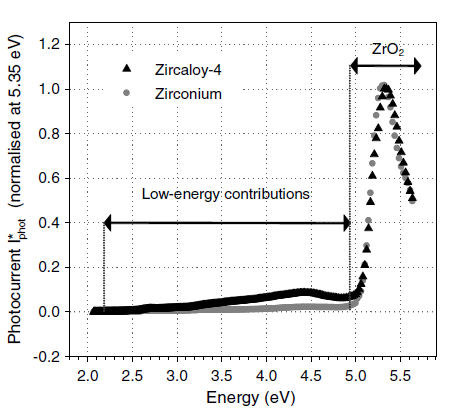
\includegraphics[width=\textwidth]{./src/figures/Benaboud2007-Fig4.png}
            \caption{}
            \label{fig_benaboud_minor_oxides_a}
        \end{subfigure}
        \begin{subfigure}{\coef\textwidth}
            \centering
            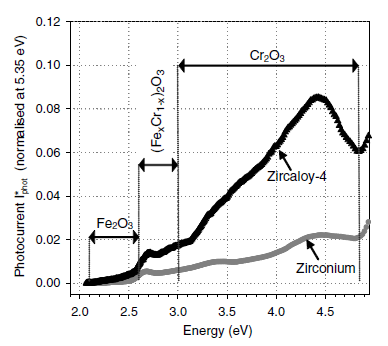
\includegraphics[width=\textwidth]{./src/figures/Benaboud2007-Fig5.png}
            \caption{}
            \label{fig_benaboud_minor_oxides_b}
        \end{subfigure}
        
        \caption{Photocurrent spectra measured on zirconia oxide layer formed on 
        Zircaloy4 and “pure” zirconium oxidized for 1h at 470°C in oxygenated 
        atmosphere\citep{benaboud2007}: a) complete spectrum b) close-up view on the minor contributions.}
        \label{fig_benaboud_minor_oxides}
    \end{figure}


\end{frame}

\subsection{Semiconduction type}
\begin{frame}{Identification of minor oxides}

\end{frame}

\subsection{High temperature PEC}





% BIBLIOGRAPHY
\begin{frame}[allowframebreaks=0.9]{References}
\AtNextBibliography{\tiny}
\nocite{*}
\printbibliography
\end{frame}

\end{document}
